% This is LLNCS.DEM the demonstration file of
% the LaTeX macro package from Springer-Verlag
% for Lecture Notes in Computer Science,
% version 2.4 for LaTeX2e as of 16. April 2010
%
\documentclass{llncs}
\usepackage[portuguese,english]{babel}
\usepackage[latin1]{inputenc}
\usepackage{url}
%\usepackage{tikz}
%\usetikzlibrary{shadows}
%\usetikzlibrary{shapes}
\usepackage{gnuplot-lua-tikz}
\usepackage{graphicx,latexsym} 
\usepackage{amssymb,amsmath}
\usepackage{longtable} 

\usepackage{acronym}
\newcommand{\listofacronymsname}{Acronyms}{}

%\usepackage{pxfonts}
%$\usepackage{url}
%\usepackage{natbib}
%\usepackage{listings}
%\usepackage{epigraph}
%\usepackage{lscape}
%\usepackage{subfigure}
%\usepackage{bibentry}
%\usepackage{subtable}

\usetikzlibrary{fit}					% fitting shapes to coordinates
\usetikzlibrary{backgrounds}	% drawing the background after the foreground
\usetikzlibrary{positioning}

\usepackage{multirow}
\usepackage{algorithmic}
\usepackage{algorithm}
%\usepackage{times}

% extremamente poderosos comandos
\def\x{{\mathbf x}}
\def\R{\mbox{\protect\makebox[.15em][l]{I}R}}
\def\w{{\mathbf w}}
\def\cbw{{\cal{\w}}}
\def\y{{\mathbf y}}
\def\t{{\mathbf t}}
\def\I{{\mathbf I}}
\def\A{{\mathbf A}}
\def\bfi{{\mathbf{\phi}}}
\def\C{{\mathbf C}}
\def\bFI{{\mathbf \Phi}}
\def\L{{\cal{L}}}
\def\N{{\cal{N}}}
\def\v{{\mathbf v}}
\def\d{{\mathbf d}}
\def\u{{\mathbf u}}
\def\z{{\mathbf z}}
\def\n{{\mathbf n}}
\def\m{{\mathbf m}}
\def\bmu{{\bm{\mu}}}
\def\bma{{\bm{\alpha}}}

%rojo? vermejo?
\def\rojo{{\color{red}}}
\newcommand{\ttf}{\ttfamily}
\newcommand{\sls}{\slshape}

\def\ba{\mathbf{\alpha}}
\newcommand{\tb}{\textbf}
\newcommand{\bi}{\begin{itemize}}\newcommand{\ei}{\end{itemize}}
\newcommand{\be}{\begin{enumerate}}\newcommand{\ee}{\end{enumerate}}
\newcommand{\bs}{\begin{slide}}\newcommand{\es}{\end{slide}}
\newcommand{\bc}{\begin{center}}\newcommand{\ec}{\end{center}}
\newcommand{\beq}{\begin{equation}}\newcommand{\eeq}{\end{equation}}
\newcommand{\beqn}{\begin{eqnarray}}\newcommand{\eeqn}{\end{eqnarray}}
\newcommand{\btab}{\begin{tabular}}\newcommand{\etab}{\end{tabular}}



\def\Y{{\mathbf Y}}
\def\X{{\mathbf X}}
\def\D{{\mathbf D}}

%JC
 \newcommand{\tab}{\hspace*{1.5em}}



\newcommand{\tikzvar}[2]{%
    \newlength{#1}
    \setlength{#1}{#2}
}

%
\urldef{\mailsa}\path|noel@ipg.pt|
\urldef{\mailsb}\path|bribeiro@dei.uc.pt|
\urldef{\mailsc}\path|jcgonc@student.dei.uc.pt|

%
\begin{document}
%
\title{Multi-Threaded Support Vector Machines For Pattern Recognition}
%


% abbreviated title (for running head) also used for the TOC unless \toctitle is used
\titlerunning{Multi-Threaded SVM for Pattern Recognition}



% the name(s) of the author(s) follow(s) next
\author{Jo\~ao Gon\c{c}alves$^{1}$ \and Noel Lopes$^{1,2}$ \and Bernardete Ribeiro$^{1}$}
%
\authorrunning{Gon\c{c}alves and Lopes and Ribeiro}   % abbreviated author list (for running head)
%
\institute{$^{1}$CISUC, Department of Informatics Engineering, University of Coimbra, Portugal \\ % \url{http://www.cisuc.uc.pt/}
%\and
$^{2}$UDI/IPG - Research Unit, Polytechnic Institute of Guarda, Portugal \\  
\mailsc, \mailsa, \mailsb
}
\maketitle              % typeset the title of the contribution

%\chapter{Acronyms}

%\listofacronyms

%\begin{acronym}
\newacro{AI}		{Artificial Intelligence	}
\newacro{ALU}		{Arithmetic and Logic Unit}
\newacro{ANN}		{Artificial Neural Network}
\newacro{API}		{Application Programming Interface}
\newacro{CC}		{Compute Capability}
\newacro{CGA}		{Colour Graphics Adapter}
\newacro{CGI}		{Computer Generated Imagery}
\newacro{CPU}		{Central Processing Unit}
\newacro{CUDA}		{Compute United Device Architecture}
\newacro{DAC}		{Digital-to-Analogue-Converter}
\newacro{DDR}		{Double-Data-Rate}
\newacro{FN}		{False Negative}
\newacro{FPR}		{False Positive Rate}
\newacro{FPS}		{First Person Shooter}
\newacro{FPU}		{Floating Point Unit}
\newacro{FP}		{False Positive}
\newacro{GLSL}		{Graphics Library Shading Language}
\newacro{GPGPU}	{General-Purpose computing on Graphics Processor Units}
\newacro{GPU}		{Graphics Processing Unit}
\newacro{HDR}		{High-Definition-Rendering}
\newacro{HLSL}		{High Level Shading Language}
\newacro{IDCT}		{inverse Discrete Cosine Transform}
\newacro{ILP}		{Instruction-Level-Parallelism}
\newacro{KKT}		{Karush-Kuhn-Tucker}
\newacro{LSB}		{Least-Significant Bit}
\newacro{NN}		{Neural Network}
\newacro{OPENCL}	{Open Computing Language}
\newacro{OPENGL}	{Open Graphics Library}
\newacro{RAMDAC}	{RAM Digital-to-Analogue-Converter}
\newacro{RAM}		{Random Access Memory}
\newacro{RBF}		{Radial Basis Function}
\newacro{ROC}		{Resource Operating Characteristic}
\newacro{SFU}		{Special Function Unit}
\newacro{SIMD}		{Single Instruction Multiple Data}
\newacro{SIMT}		{Single Instruction Multiple Thread}
\newacro{SISD}		{Single Instruction Single Data}
\newacro{SMO}		{Sequential Minimal Optimization}
\newacro{SMP}		{Symmetric-Multi-Processing}
\newacro{SM}		{Streaming Multiprocessor}
\newacro{SPMD}		{Single Process Multiple Data}
\newacro{SP}		{Shading Processor}
\newacro{SVM}		{Support Vector Machine}
\newacro{TN}		{True Negative}
\newacro{TPC}		{Thread Processing Cluster}
\newacro{TPR}		{True Positive Rate}
\newacro{TP}		{True Positive}
\newacro{UMA}		{Uniform Memory Access}
\newacro{UKF}		{Universal Kernel Function}
\newacro{VLIW}		{Very Long Instruction Word}
\newacro{VPU}		{Video Processor Unit}
\newacro{VR}		{Virtual Reality}
\newacro{TNR}		{True Negative Rate}
\newacro{FDR}		{False Discovery Rate}
\newacro{MCC}		{Matthews Correlation Coefficient}
\newacro{SV}		{Support Vector}
%\end{acronym}


\begin{abstract}
Support Vector Machines (SVM) have become indispensable tools in the area of pattern recognition. They show powerful classification and regression performance in highly non-linear problems by mapping the input vectors
nonlinearly into a high-dimensional feature space through a kernel function. However, the optimization task is numerically expensive since single-threaded implementations are hardly able to
cope up with the complex learning task. In  this paper, we present a multi-threaded implementation of the Sequential Minimum Optimization (SMO) which reduces the numerical complexity by parallelizing the KKT conditions update, the calculus of the hyperplane offset and the classification task.
Our preliminary performance results in a few benchmark datasets and in a MP3 steganalysis problem are competitive compared to state-of-the-art tools while the execution running times were considerably faster. 
\keywords{SVM, OpenMP, sequential minimum optimization (SMO)}
\end{abstract}
%

%includes Karush Kuhn Tucker (KKT) conditions update, a first order heuristic search and the  calculus of hyperplane offset b, and the classification process



\section{Introduction}
The increasing complexity and performance demands in pattern recognition applications require innovative and fast approaches to cope with the system non-linearities.  In particular, the design  of efficient and scalable systems depends on powerful tools  to extract relevant (and meaningful) information.   Additionally, the learning algorithms often require high-processing capabilities  making current single-threaded algorithms  unable to scale with the demanding processing power needed. Among the supervised learning algorithms, \acp{SVM} are the most widely used algorithm due to their generalization properties and regularizatizon capability. \acp{SVM} are binary large margin classifiers which have found successful applications in many scientific fields such as engineering and bioinformatics~\cite{ZieRaeMikSchLenMue00}, information management~\cite{Ando2005}, finance and business~\cite{Wu2010} among many others.   
The \ac{SVM} aims to find the optimal decision hyperplane which is equivalent  to reach both the smallest generalization and empirical errors. This method shows powerful classification and regression performance in complicated nonlinear problems by using the Mercer kernel function which transforms the input vectors into a highly-dimensional space and by learning a linear  model in this feature space.  
An important and crucial point in the \ac{SVM} formulation is that it can provide a good generalization independent of the training set's distribution by making use of the principle of structural risk minimization~\cite{Vapnik1995,CorVap95}.
However, they usually require significant memory and computational burden for calculating the large Gram matrix~\cite{Chen2012}. To lift this limitation some fast learning methods have been studied~\cite{Suykens2010,Suykens2005}. However, most of these algorithms do no take into account the multi-cores avalaible today in CPU baseline computers.
In this paper we focus on a multi-threaded CPU  standalone SVM version (MT-SVM)  which builds up from the scratch an implementation of the Sequential Minimal Optimization(SMO) algorithm and is characterized by being paralellized.  
Although previous approaches have been developed~\cite{Catanzaro2008}, our implementation includes a new kernel function, the Universal Kernel Function (UKF)~\cite{Rui2011} which leads to a broad spectrum of the generalization capabilities of the learning machine. Experiments performed on UCI datasets benchmarks~\cite{Asuncion2010} yield performance competitive results as compared to state-of-the-art LIBSVM tools while delivering  better speedups. In the grounds of a real world MP3 steganalysis high-dimensional problem which aims at discovering hidden audio messages the algorithm runs fast and the speedups obtained are excellent.  %(\cite{cit:Ferrer2005} )

The paper is organized as follows: Section~\ref{sec:svm} describes the \ac{SVM} training and classification tasks. Section~\ref{sec:svm_smo} addresses the \ac{SMO} algorithm. Section~\ref{sec:svm_psmo} describes the parallel implementation of both the training and classification tasks. We present our results in section~\ref{sec:exp_results}. The conclusions as well as future work are addressed in section~\ref{sec:conclusions}.

\section{Support Vector Machines (SVM)}
\label{sec:svm}
\subsection{Preliminarities}
\label{sec:svm_formulation}
Given a set of $n$ training points in a $d$ dimensional feature space $(\x \in R^d)$ each associated with a label $(y_i \in \{-1, 1\})$ the binary soft-margin kernel \ac{SVM} solves the linearly convex quadratic problem:
%-------
%\begin{alignat}{2}
%	\label{eq:svm_min_w}
%	\text{minimize}   & \qquad	\frac{1}{2}\Arrowvert \textbf{w} \Arrowvert ^2 + C \sum\limits_{i=1}^{n}\xi_i &&\qquad	\\ 
%	\label{eq:svm_constraints}
%	\text{subject to} & \qquad \xi \geq 0 &&\qquad \\
%	& \qquad	y_i(\textbf{w}\cdot\textbf{x}_i+b)\geq 1 - \xi_i, &\qquad	& i=1,2,\dots n
%\end{alignat}
%%-------
%Which has the following dual:
%-------
\begin{align}
	\label{eq:svm_kernel_dual1} \text{maximize} \quad & \sum\limits_{i=1}^{n} \alpha_i - \frac{1}{2} \sum\limits_{i=1}^{n} \sum\limits_{j=1}^{n} \alpha_i\alpha_j y_i y_j K(\x_i,\x_j) \\
	\label{eq:svm_kernel_dual2} \text{subject to} \qquad & \sum\limits_{i=1}^{n} \alpha_i y_i = 0 \\
	\label{eq:svm_kernel_dual3} \text{and} \qquad & 0 \leq \alpha_i \leq C, \qquad i=1,2,\dots n
\end{align}
%-------
For each training point $\x_i$ there is an associated Lagrange multiplier $\alpha_i$. These multipliers are bounded by two limits (equation \ref{eq:svm_kernel_dual3}) where $C$ is the penalization constant. The careful selection of this constant allows the \ac{SVM} to balance the generalization  and empirical error on the training set. In practical terms this is equivalent to control the size of the gap between both training classes. The data points which have $\alpha_i > 0$ are the \acp{SV} and define the decision boundary. After convergence the offset $b$ is calculated as a weighted arithmetic average using the SVs, where in (equation \ref{fig:svm_b_calculus}) $n_{SV}$ is the number of support vectors:
\begin{align}
%b=\frac{b_{low}+b_{high}}{2}
b=\frac{1}{n_{SV}}\sum\limits_{j=1}^{n_{SV}} \left( \sum\limits_{i=1}^{n} \alpha_i y_i K(\x_i,\x_j) \right) -y_j
\label{fig:svm_b_calculus}
\end{align}
To improve performance on non-linearly separable classes, the above optimization task (equation \ref{eq:svm_kernel_dual1}) makes use of the kernel trick which allows the \ac{SVM} to work on a higher dimension feature space by means of a dot-product between two vectors $\x_i$ and $\x_j$. This result is calculated using the kernel projection $K(\x_i,\x_j)$. Therefore with a non-linear kernel the margin corresponds to a non-linear boundary in this new feature space.
The standard kernel functions (linear, polynomial, gaussian and sigmoid) are available in our implementation. Moreover, a recent kernel function, Universal Kernel Function (UKF)~\cite{Rui2011}which has found successful applications in various domains is also considered. %isto esta bem?
\begin{equation}
K(\u,\v) = \displaystyle L (\|\u - \v \|^2 + \sigma^2)\displaystyle^{\displaystyle-\alpha}
\end{equation}
This kernel aims to gather points near to each other, in a higher dimension space, since they are strongly correlated. Therefore it can provide a smaller number of SVs and thus fasten both the training and classification tasks. Additionally, the UKF kernel can yield better performance generalization~\cite{Ayat02kmod}.
%isto sao quotes:
%firstly, it is not necessary to make a selection out of the above mentioned kernel functions, which can simplify the modeling process and, consequently, will save a lot of computing time; secondly, it has a stronger mapping ability and can properly deal with a large variety of mapping problems due to its flexibility to vary.
%the UKF kernel can lead to improve classification accuracy. This strongly suggests that application of the UKF kernel can improve the generalization performance of SVM greatly.

Finally, the classification of a given sample $\z$ is done using a subset of the training set - the support vectors. The \ac{SVM}'s classification task is:
\begin{equation} \label{eq:svm_kernel_classfc}
y(\z)=\text{sign} \left( b + \sum\limits_{i=1}^{n}\alpha_i y_i K(\x_i,\z)\right)
\end{equation}
\section{Sequential Minimal Optimization (SMO) Algorithm }
\label{sec:svm_smo}
%se calhar e melhor remover isto?
Previous computational methods to solve the training problem are slow because they are based on Numerical Optimization libraries, in the form of third-party QP solvers. Additionally, they require high amounts of memory to solve the task at hand. There are better alternatives like by working in chunks of training samples~\cite{Vapnik1995} or by decomposing the problem into a series of smaller QP sub-problems~\cite{Osuna1997,Platt1998}.
Platt developed in 1998 the Sequential Minimal Optimization(SMO) algorithm.
%This algorithm is based on Osuna's decomposition scheme and solves the smallest possible optimization task at each step, updating two $\alpha$ variables.
At each step, only the two $\alpha$ variables are required to be solved, because the function to be optimized (equation \ref{eq:svm_kernel_dual1}) has in its definition
two Lagrange multipliers, $\alpha_i$ and $\alpha_j$. Additionally, both multipliers must satisfy one linear constraint (equation \ref{eq:svm_kernel_dual2}) and must be in the range given by equation \ref{eq:svm_kernel_dual3}~\cite{Platt1998,Catanzaro2008}.
The main steps of the soft-margin \ac{SMO} algorithm with the kernel trick are described detailed in Algorithm~\ref{algo:smo}~\cite{Catanzaro2008,L.J.Cao2006}.
%-------
\begin{algorithm}
\caption{Sequential Minimum Optimization (SMO) algorithm}
\label{algo:smo}
\algsetup{indent=5em}
\begin{algorithmic}[1]
\REQUIRE $\x_i\in\chi$, $y_i\in\Omega$, $i\in\{1\cdots n\}$
\STATE Initialize: \\
$\alpha_i$=0, $f_i$=$-y_i$, $\forall i \in\{1\cdots n\}$ \\
\STATE Initialize: \\
$ b_{high} = -1 $, $ b_{low} = 1 $, $ i_{high} = \text{min}\{i:y_i=1\} $, $ i_{low} = \text{min}\{i:y_i=-1\}$, \\ $\forall i \in\{1\cdots n\}$
\STATE Update: $\alpha_{i{low}}$, $\alpha_{i_{high}}$
\REPEAT
	\STATE Update optimality conditions $f_i$
	\STATE Compute: $b_{high}$, $b_{low}$, $i_{high}$, $i_{low}$
	\STATE Update $\alpha_{i_{low}}$, $\alpha_{i_{high}}$, $\forall i \in\{1\cdots n\}$
\UNTIL{$b_{low}\leq b_{high} + 2\tau$}
\end{algorithmic}
\end{algorithm}
%-------
The whole set of $\alpha_i$ are initialized to $0$ as they satisfy the constraints defined in equation \ref{eq:svm_kernel_dual3}. In each step, after choosing $i_{high}$ and $i_{low}$, the new values for the two Lagrange multipliers $\alpha_i^{\text{new}}$ are computed as follows:
%-------
\begin{align}
\alpha_{i_{low}}^\text{new} & = \alpha_{i_{low}} + y_{i_{low}} \frac{b_{high}-b_{low}}{\eta} \\
\alpha_{i_{high}}^\text{new} & = \alpha_{i_{high}} + y_{i_{low}}y_{i_{high}} (\alpha_{i_{low}}-\alpha_{i_{low}}^\text{new})
\end{align}
%-------
where $\eta$ is defined as:
%-------
\begin{equation}
\eta = K(x_{i_{high}},x_{i_{high}})+K(x_{i_{low}},x_{i_{low}})-2\cdot K(x_{i_{high}},x_{i_{low}})
\end{equation}
%-------
%As described by Platt, $\eta$ can be non positive if a given kernel $K$ does not obey Mercer's conditions. Because this work does not have this kind of kernels, this condition is not handled. %ref do artigo do PLATT
Naturally, both $\alpha_{i_{low}}$ and $\alpha_{i_{high}}$ must satisfiy equation~\ref{eq:svm_kernel_dual3}. If $\alpha_{i_{low}}$ changes by $\delta$ then $\alpha_{i_{high}}$ changes by the same amount on the opposite direction ($- \delta$), because of the constraint defined in equation~\ref{eq:svm_kernel_dual2}. Next, the \ac{KKT} conditions must be updated for each sample $\x_i$ using:
%-------
\begin{equation}
%f_i=\w(\alpha)\cdot \z_i-y_i = \sum\limits_{j=1}^{d}\alpha_i y_i K(\x_i,\x_j)-y_i
f_i= \sum\limits_{j=1}^{n}\alpha_i y_i K(\x_i,\x_j)-y_i
\end{equation}
%-------
which can be simplified to:
%-------
\begin{equation}
f_i=f_i^{old}+(\alpha_{i_{high}}^{new}-\alpha_{i_{high}})y_{i_{high}}K(x_{i_{high}},x_i) + (\alpha_{i_{low}}^{new}-\alpha_{i_{low}})y_{i_{low}}K(x_{i_{low}},x_i)
\end{equation}
%-------
The indices of the next Lagrange multipliers $ i_{low} $ and $ i_{high} $ are chosen from two corresponding sets:
\begin{align}
I_{low} &= \{i:0<\alpha_i<C\} \cup \{i:y_i>0 , \alpha_i=C\} \cup \{i:y_i<0 , \alpha_i=0\} \\
I_{high} &= \{i:0<\alpha_i<C\} \cup \{i:y_i>0 , \alpha_i=0\} \cup \{i:y_i<0 , \alpha_i=C\}
\end{align}
The optimality coefficients $b_{low}$ and $b_{high}$ are calculated as:
\begin{align}
b_{low}=\text{max}\{f_i:i\in I_{low}\} \\
b_{high}=\text{min}\{f_i:i\in I_{high}\}
\end{align}
For simplicity, to choose $i_{low}$ and $i_{high}$ we use the first order heuristic~\cite{Keerthi2001}. For the next iteration, these indices are calculated as:
\begin{align}
i_{low}&=\text{arg max}\{f_i:i\in I_{low}\} \\
i_{high}&=\text{arg min}\{f_i:i\in I_{high}\}
\end{align}
The algorithm is executed while the following holds:
\begin{align}
b_{low}\leq b_{high} + 2\tau \Leftrightarrow b_{low} - b_{high} \leq 2\tau
\end{align}
where $\tau : 0<\tau<1$ is the tolerance of the solution's optimality and in fact the stopping criteria. After converging, the parameter $b$ can be calculated: either as an arithmetic mean between $b_{low}$ and $b_{high}$ or as a weighted average using the SVs. The latter  (equation~\ref{fig:svm_b_calculus}) is more precise, therefore it will be used here. %esta ultima frase soa mal
\section{Parallel SMO implementation}
\label{sec:svm_psmo}
Our implementation was developed in \texttt{C++} using OpenMP. This \acs{API} allows developers to write multi-threaded shared memory (also named \ac{UMA}) applications in either C/C++ or Fortran. Programs written using this approach are in Flynn's taxonomy classified as \ac{SPMD} because the same program is executed by different threads (cores) but each processing a different subset of the data.
%se calhar e melhor cortar-se isto
%The OpenMP library uses the fork-join model of parallel execution where programs begin as a single process: the  master thread.  The master thread executes sequentially until the first parallel region construct is encountered. Shortly, the execution is split by multiple threads and in the end of the region the master threads waits for the arrival of the other threads.

Even though the SMO algorithm is in its essence sequential our emphasis is that there are steps which can be safely parallelized. In fact, these steps match the areas where most of the computation is done and, therefore, where the algorithm  consumes more time~\cite{L.J.Cao2006,Catanzaro2008}. One of such steps can be easily identified as the \ac{KKT}'s conditions update (using $f_i$ and the kernel Gram matrix), which is the costliest arithmetic step in the \ac{SMO} algorithm, as noticed in~\cite{L.J.Cao2006}. This corresponds to what is known as an embarrassingly parallel task, because the calculus of each $f_i$ is independent of each other. Consequently, it fits nicely to the multi-core \ac{CPU} architecture.

Another phase which can be fastened is the computation of the next $b_{low}$, $b_{high}$, $\alpha_{low}$ and $\alpha_{high}$. As this is done by performing a first order heuristic search, it can be executed in parallel using the well-known reduction operations \textit{min} and \textit{max}. Each thread works on a subset of both $I_{high}$ and $I_{low}$ and finds locally the variables specified in the beginning of this paragraph. The master thread waits for the other thread's results and then applies the reduction operators. The calculus of offset $b$ is also implemented in parallel for each SV. The only sequential steps are the Lagrange multipliers ($\alpha_{i{low}}$ and $\alpha_{i_{high}}$) update and the convergence verification (step 5 on algorithm \ref{algo:smo}).

%esta palavra 'in' diz que esta mal, mas nao percebo
The above parallel tasks are divided into equal parts, each one assigned to a corresponding thread. In theory, if the original single-threaded \ac{SMO} training process takes $T_s$ time, using a processor with $P$ cores, the multi-threaded \ac{SMO} would execute in $T_p = \frac{T_s}{P}$ and offer a speedup of $P \times$. However, this theoretical speedup is rarely achieved in practice because part of the code is not parallelized. Even though the algorithm can be fully parallel, the sequential sections always exist (Amdahl's law) due to: (i) synchronization, where some threads must wait for the completion of others, (ii) memory bandwidth, which is shared by all CPU cores, and (iii) mutual exclusion areas, among other reasons.
\section{Experimental Setup, Results and Discussion}
\label{sec:exp_results}
In order to evaluate our MT-SVM implementation w.r.t. the performance and speedup we compared the results in  benchmarks and in the MP3 steganalysis dataset with the state-of-the-art LIBSVM~\cite{Chang2011} (version 3.11). Both tools use the SMO algorithm. 
For fairness we set LIBSVM's cache to one MegaByte since currently our implementation does not make use of a kernel cache. Unless specified, we set the number of threads to $4$ in our implementation. The system used for testing has an Intel Quad Core i5-750 processor with the clock set to 3.33 GHz. The machine also has 12 GB RAM.
%----
\begin{table}
	\begin{center}
\caption{Datasets and RBF kernel $\gamma$ parameter used in the experiments.}
\label{table:datasets}
		\begin{tabular}{ | l | c | c | c | }
		\hline
		Dataset & \#Samples & \#Features & $\gamma$ \\ \hline \hline
		\hline
		Adult &			32561 &	14 & 0.1\\  
		Breast Cancer Wisconsin - Diagnostic (wdbc) &	569   &	30 & 0.1\\ 
		Two-Spiral (spiral) & 		2097152  &	2  & 12.5\\ \hline
		MP3 Steganalysis (stego) & 		1994  &	742  & 0.001\\ \hline
		\end{tabular}
	\end{center}
\end{table}

%-------
At this point our implementation is designed exclusively for binary tasks, thus we have specifically chosen binary class datasets for the experimental setup. Two datasets are available from the UCI Machine Learning repository\footnote{~\url{http://archive.ics.uci.edu/ml/}}.
%-------------(see Figure~\ref{fig:results:spiral_plot})
The Two-Spiral dataset consists of learning to discriminate between data distributed on two distinct spirals that coil around each other in the x-y plane. It was built in order to assess the \ac{UKF} kernel efficiency. We tested the \ac{UKF} kernel against  the \ac{RBF} kernel, with the following settings: $L = 2.0$, $\sigma = 0.6$ and $\alpha = 14.0$.  
 
%----------
The MP3 Steganalysis dataset was extracted from a real problem using the four methods described in~\cite{Qiao2009}. The dataset is composed of two classes: the first corresponds to normal MP3 audio files (cover) and the second are the same MP3 files with hidden information (stego). %The data was kindly provided by X. OU the authors thanks..?
%----------

%\begin{figure}
%	\centering
%	\caption{Scatter plot of the dataset ``Spiral''.}
%	\vspace{0.333cm}
%	\includegraphics[width=0.666\textwidth]{pictures/spiral_2m_scatterplot.png}
%	\label{fig:results:spiral_plot}
%\end{figure}
Table~\ref{table:datasets} lists the main characteristics of the datasets. The datasets were normalized before being processed using a standard score procedure. % which normalizes each sample ($\x$) according to the population's mean ($\bar{\x}$) and standard deviation ($\sigma$). 
Otherwise stated, the kernel used in the experiments was the \ac{RBF} kernel. This table also presents the $\gamma$ parameter used in the \ac{RBF} kernel. We set the parameter $\gamma$ by using a grid search in order to obtain the best classification performance. The penalization constant $C$ was set to $1$ and the optimality gap $\tau$ was set to $0.01$ in all the tests performed. We ran the experiments $10$ times for each dataset with 5-fold cross validation. Consequently, each classifier was run $50$ times.  I/O times are excluded.

%--------------
\begin{table}[!ht]
  \centering
  \caption{Mean values of Accuracy and F-Score with MT-SVM and LIBSVM.}
    \begin{tabular}{|l|r|r|r|r|r|r|} \hline
    Dataset & MT-SVM & LIBSVM & MT-SVM & LIBSVM & Accuracy & F-Score \\
          & \multicolumn{2}{|c|}{Accuracy (\%)} & \multicolumn{2}{|c|}{F-Score (\%)} & \multicolumn{2}{|c|}{Improvement (\%)} \\ \hline
    adult & 84.63 & 84.72 & 90.12 & 90.38 & $\downarrow$ 0.09 & $\downarrow$0.26 \\
    wdbc  & 95.71 & 95.85 & 94.33 & 94.49 & $\downarrow$0.14 & $\downarrow$0.16 \\
    spiral & 100.00 & 100.00 & 100.00 & 100.00 & 0.00  & 0.00 \\ \hline
    stego & 97.05 & 96.92 & 97.00 & 97.00 & $\uparrow$ 0.13  & 0.00 \\ \hline
    \end{tabular}
  \label{tab:results_classification_acc_fscore}
\end{table}

As illustrated in Table \ref{tab:results_classification_acc_fscore}  MT-SVM yields competitive performance as compared  to LIBSVM which obtained slightly better in both adult and wdbc data sets, in accuracy, by an increase of $0.09\%$ and $0.14\%$, and, in F-score, by an increase of  $0.26\%$ and $0.16\%$, respectively. Note that since the ``spiral'' dataset is separable in a higher feature space, both methods yield $100 \%$ of accuracy and F-Score by using the \ac{RBF} kernel. On the other hand, LIBSVM achieved a slightly worse result of $0.13\%$ in the ``stego'' dataset.

%--------------
\begin{table}[!ht]
  \centering
  \caption{Training times and total amount of iterations with MT-SVM and LIBSVM}
    \begin{tabular}{|l|r|r|r|r|r|} \hline
    Dataset & \multicolumn{2}{|c|}{MT-SVM} & \multicolumn{2}{|c|}{LIBSVM} & Speedup (x) \\ 
          & Time (s) & Iterations & Time (s) & Iterations &  \\ \hline\hline
    adult & 15.93 & 15358.50 & 32.49 & 11124.46 & $\uparrow$ 2.04 \\
    wdbc  & 0.04  & 286.10 & 0.06  & 254.94 &  $\uparrow$ 1.80 \\
    spiral & 24.86 & 594.00 & 180.07 & 1076.76 & $\uparrow$ 7.24 \\ \hline
    stego & 0.33 & 465.18 & 1.17 & 377.86 & $\uparrow$ 3.59 \\ \hline
    \end{tabular}
  \label{tab:results_training}
\end{table}

We also illustrate  in Table~\ref{tab:results_training} the higher speedups obtained by MT-SVM as compared to LIBSVM which cover the range ($1.8 - 7.24$)$\times$. This is clearly evidenced by the maximum speedup of $7.24\times$ of  our method over LIBSVM obtained in the spiral data set. This might be in partly due to the large number of iterations  performed by LIBSVM. For the three datasets LIBSVM's heuristics are effective in accelerating the training convergence. Using the adult dataset the speedup obtained by our version against LIBSVM ($2.04\times$) is similar to the one obtained by~\cite{L.J.Cao2006} using four processors ($2.17\times$).

%For training we obtained speedups of the order $1.8-7.24\times$ although the slower performance obtained by  on the spiral dataset most likely can be attributed to its second heuristic search. %esta afirmacao e melhor cortar, pois nao tenho a certeza.
%--------------
\begin{table}[!ht]
  \centering
  \caption{Number of Support Vectors (SVs) used by MT-SVM and LIBSVM.}
    \begin{tabular}{|l|r|r|r|} \hline
    Dataset & MT-SVM & LIBSVM & Improvement (\%)\\
          & \#SVs & \#SVs &  \\ \hline\hline
    adult & 9818.20 & 9788.40 & $\downarrow$ 0.30 \\
    wdbc  & 186.58 & 188.00 & $\uparrow$ 0.76 \\
    spiral & 663.72 & 952.65 & $\uparrow$ 43.53 \\ \hline
    stego & 346.16 & 348.08 & $\uparrow$ 0.55 \\ \hline
    \end{tabular}
  \label{tab:results_svs}
\end{table}

The number of SVs for the adult, wdbc and stego datasets for both our implementation (MT-SVM)  and LIBSVM are similar (see Table \ref{tab:results_svs}) although there is a slight improvement using our tool. For the spiral dataset LIBSVM the number of SVs is increased by $43.53 \%$.
% probably due to the same reason as mentioned above.
%--------------
\begin{table}[!ht]
  \centering
  \caption{Classification times used by MT-SVM and LIBSVM.}
    \begin{tabular}{|l|r|r|r|} \hline
    Dataset & MT-SVM & LIBSVM & Speedup (x) \\
          & Time (s) & Time (s) &  \\ \hline\hline
    adult & 0.89  & 3.02  & $\uparrow$ 3.40 \\
    wdbc  & 0.01  & 0.07  & $\uparrow$ 6.02 \\ 
    spiral & 3.01  & 11.65 & $\uparrow$ 3.87 \\ \hline
	stego & 0.02 & 0.09 & $\uparrow$ 3.92 \\ \hline
    \end{tabular}
  \label{tab:results_classification}
\end{table}

According to Table~\ref{tab:results_classification} the classification speedup is almost linear with the amount of used threads (four), excluding the ``wdbc'' dataset. This is explained by the fact that the classification task is inherently parallel.
%LIBSVM classification on the ``wdbc'' dataset was slower, very likely because of additional processement done by the program when compared to ours.

%--------------
\begin{table}[!ht]
  \centering
  \caption{Speedup for both the training and classification tasks achieved by MT-SVM with the amount of threads for the ``adult'' dataset.}
    \begin{tabular}{|c|c|c|c|c|} \hline
    Number of threads & Classification (s) & Training (s) & Classification (x) & Training (x) \\ \hline
    1     & 3.29  & 51.01 & 1.00  & 1.00 \\ \hline
    2     & 1.65  & 27.75 & 1.99  & 1.84 \\ \hline
    3     & 1.10  & 19.62 & 2.98  & 2.60 \\ \hline
    4     & 0.89  & 15.93 & 3.70  & 3.20 \\ \hline
    \end{tabular}
  \label{tab:results_speedup_vs_cores}
\end{table}%

Table \ref{tab:results_speedup_vs_cores} and Figure \ref{fig:results:cores_vs_speedup} reflects the efficiency of our algorithm with the amount of threads, for the ``adult'' dataset. Our implementation is faster than LIBSVM when running with two or more threads (Table~\ref{tab:results_training} and Table~\ref{tab:results_classification}) in both training and classification tasks. When using up to four threads the speedup achieved by our algorithm is almost linear with the number of threads.

\begin{figure}[!ht]
	\centering
	\caption{Scatter plot of the ``adult'' dataset.}
	\vspace{0.333cm}
	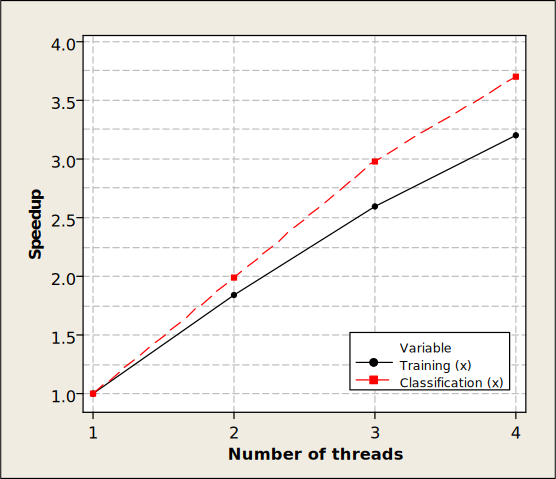
\includegraphics[width=0.666\textwidth]{pictures/mysvm_mt_cores_vs_speedup.pdf}
	\label{fig:results:cores_vs_speedup}
%	\line(1,0){425}
\end{figure}

% Table generated by Excel2LaTeX from sheet 'rbf vs ukf'
\begin{table}[!ht]
  \centering
  \caption{UKF kernel performance compared against the RBF kernel when using the ``adult'' dataset.}
    \begin{tabular}{|r|r|r|r|r|r|} \hline
    Kernel & Implementation & Classification (s) & Training (s) & Training iterations & \#SVs \\ \hline
    UKF   & MT-SVM & 2.82  & 12.88 & 173.01 & 333.60 \\ \hline
    RBF   & MT-SVM & 3.01  & 24.86 & 594.01 & 663.72 \\ \hline
    RBF   & LIBSVM & 11.65 & 180.07 & 1076.76 & 952.65 \\ \hline
    \end{tabular}%
  \label{tab:ukf_vs_rbf}%
\end{table}%

Using the ``spiral'' dataset the UKF kernel gives excellent results (see Table~\ref{tab:ukf_vs_rbf}). Compared to our implementation with the RBF kernel both the total amount of iterations and training time was reduced to half, and for comparison, LIBSVM does $3\times$ more iterations than our implementation with the UKF kernel. In this situation, LIBSVM was $13.98\times$ slower than our implementation. Additionally, we also obtained $100\%$ accuracy and F-Score using the \ac{UKF} kernel.
%=================================================
\section{Conclusions and Future Work}
%=================================================
\label{sec:conclusions}
As the amount of data produced grows at an unprecedented rate, fast machine learning algorithms that can extract relevant and useful information from large repositories of data have become extremely important. To partly answer to this challenge 
in this paper we proposed a multi-threaded parallel implementation MT-SVM which parellizes the SMO algorithm. Our tool makes use of the greater power available on multi-core \acp{CPU} and efficiently learns and classifies within several domains, presenting good properties in scaling data. Speedups up to $7\times$ on training and up to $4\times$ on classification tasks were achieved.
Additionaly we included  the \ac{UKF} which has good generalization properties in the high-dimensional feature space. Although the UKF has more parameters to fine tune, depending on the dataset, both the classification and generalization performance are promising.
In future work we will add vectorization (SSE or AVX) as well as support for kernel caching which may drastically decrease the amount of computations to be performed by the algorithm. Additionally, we will develop a component in Graphics Processing Units (GPU) which might be helpful for pattern recognition applications.
%To cope with the increasingly computational performance demands, the challenge consists of building multi-core implementations of machine learning algorithms.

%When comparing the times taken with our single-threaded implementation against LIBSVM its clear their classifier is faster and also extremely optimized. But when using our version with more than two threads both the training and classifications tasks are faster. This  on computers with multi-core \acp{CPU}.

%A first step was presented in this paper with a multi-thread implementation of \ac{SVM}. The algorithm was tested on UCI benchmark datasets yield promising results as compared with well-established software in the domain of machine learning and pattern recognition. 



%=================================================
% Bibliography
%=================================================

\bibliographystyle{splncs03}
\bibliography{SVM_GPU_ciarp,estagio_ciarp}

\end{document}
